\chapter{Methodology}
\label{chap:methodology}

 
 
 \section{Project description}
 
 \begin{itemize}
  	\item Papiit
 	\item Temixco
 	\item Grafica de radiación
 	\item Hay potencial
 	\item cafetería modeling
 	\item aspersores, direct evaporative modelling, foto del osm
 \end{itemize}
 

This thesis work is a product of the Papiit project, Estudio teórico-experimental del enfriamiento evaporativo en eficicaciones.
Objetivo de Papiit. 

This project study and aim to simulate the evaporative cooling process that takes place in the sprayers located within the IER cafeteria area. As the IER is situated in Temixco, a township of the state of Morelos, the numerical experiments were carried out with local data.

 Temixco is a city located in the mexican state of Morelos, it borders with Cuernavaca and Jiutepec. It has a latitud of 18.85°, -99.22° of longitud, 1253 MSL and 89,869 $km^{2}$ of territorial extension. According to the population and housing census made in 2020 by the Instituto Nacional de Estadística, Geografía e Informática (INEGI)[1]the city has a population of 122,263 people. Its climate is form by to kinds; warm sub-humid and semi-warm sub-humid climate [2]. The temperature range is 18-24°C and the precipitation range, which most is in summer, is 800-1200 mm. 
 
\begin{figure}
 \centering
 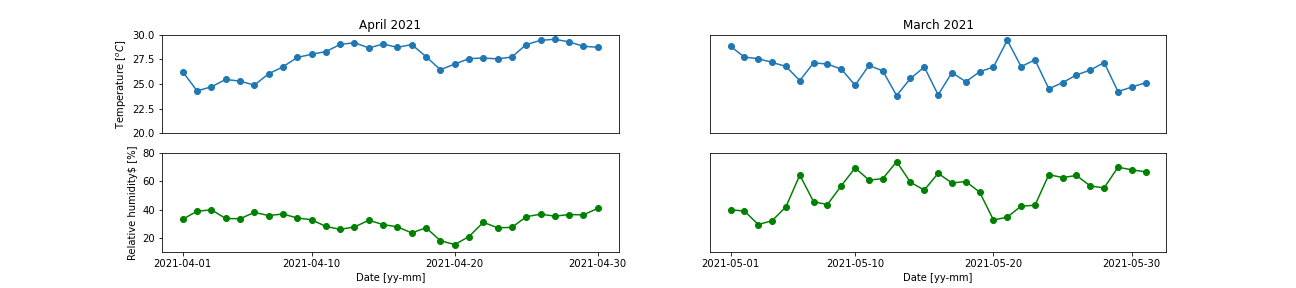
\includegraphics[scale=0.3]{tempVShum}
 \caption{	
 Mean temperature and relative humidity in March and April 2021 according to ESOLMET.
 \label{fig:tempvshum}
 }
\end{figure}

\begin{figure}
 \centering
 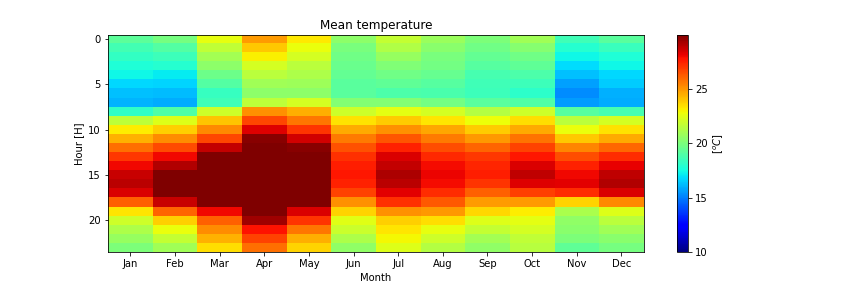
\includegraphics[scale=0.4]{Temperature}
 \caption{	
 Temperature, IER 2021 according to ESOLMET.
 \label{fig:temp}
 }
\end{figure}

\begin{figure}
 \centering
 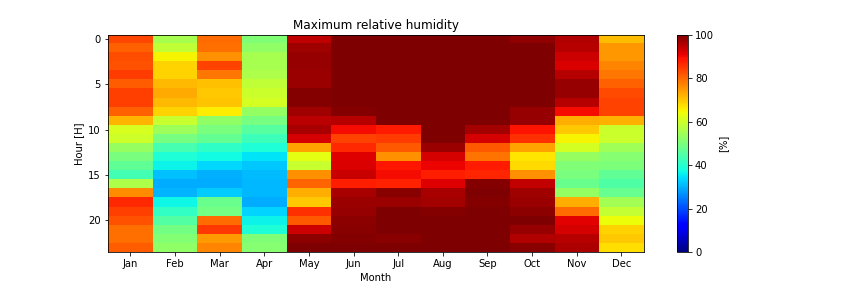
\includegraphics[scale=0.4]{relhum}
 \caption{	
 Relative humidity, IER 2021 according to ESOLMET.
 \label{fig:rh}
 }
\end{figure}


\begin{figure}
 \centering
 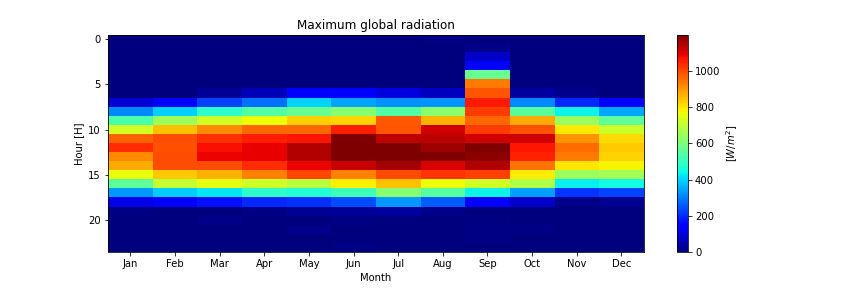
\includegraphics[scale=0.4]{Ig}
 \caption{	
 Global radiation, IER 2021 according to ESOLMET.
 \label{fig:Ig}
 }
\end{figure}

Experiments and measurements made to study evaporative cooling effect were carried out in the IER´s cafeteria in Temixco, Morelos. It corresponds the second of four stories of a rectangular building which principal façade is oriented to the east, facing Quetzalcoatl place, with an 6° angle deflected clockwise. 


The cafeteria it’s a space of constant traffic of people. Although kitchen has a schedule of 9 am to 5 pm, it is used to be people sitting there all day. However, the most crowed hours are 2-4 pm which correspond mealtime for the most people in the institute. While the number of people tends to vary according to the time and day, the human activity carried out in this space does not involve a higher charge of energy than that of people seated. Of course, this is true without involving kitchen activities.

The cafeteria is a space with 8.65 x 10 square meters of area and 3.5 meters high, without taking account the kitchen area.  The space that is described as a cafeteria is a semi-open space. It has a wall that points to the south, the half separation of the kitchen to the north, a wall with latticework to the west and the part to the east, in front of the Quetzalcoatl square, is open.

\begin{figure}
\centering
\begin{subfigure}[b]{0.45\linewidth}
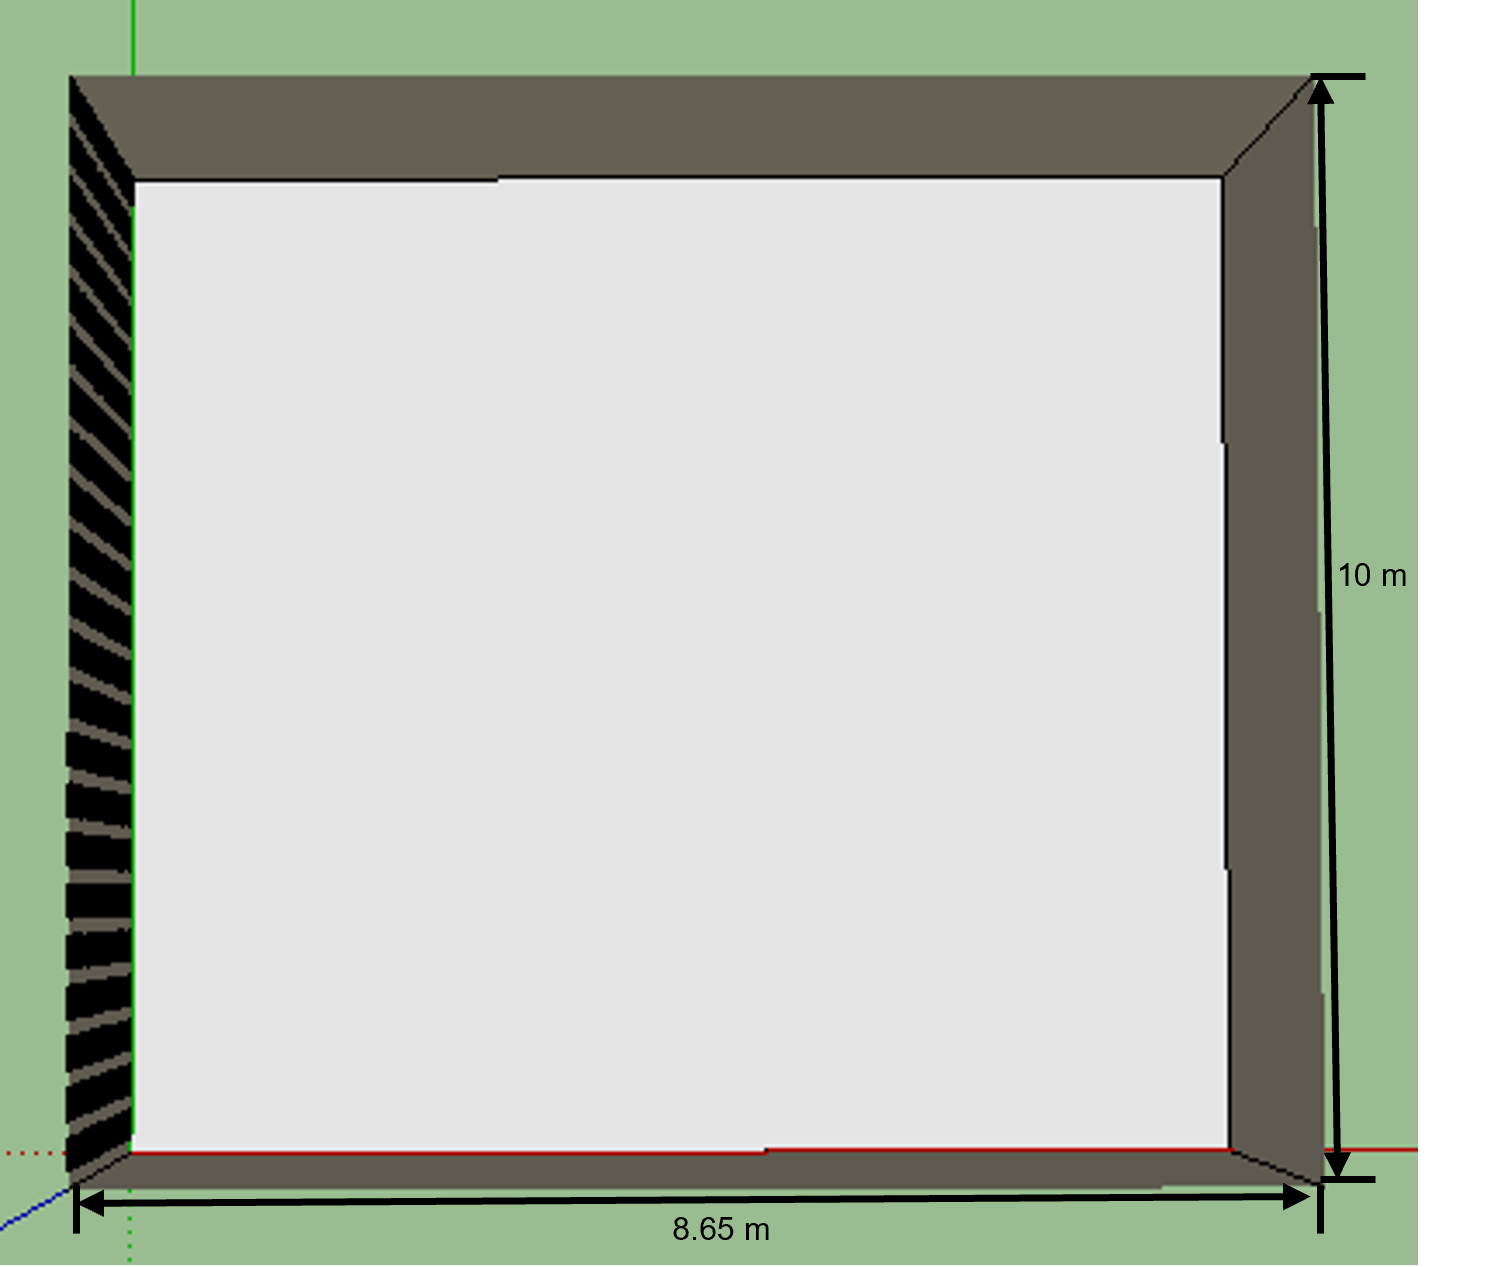
\includegraphics[scale=0.44]{cafeteriaSketch_arriba_dimesiones.PNG}
\caption{Upper view}
\label{fig:Upper view}
\end{subfigure}
\begin{subfigure}[b]{0.45\linewidth}
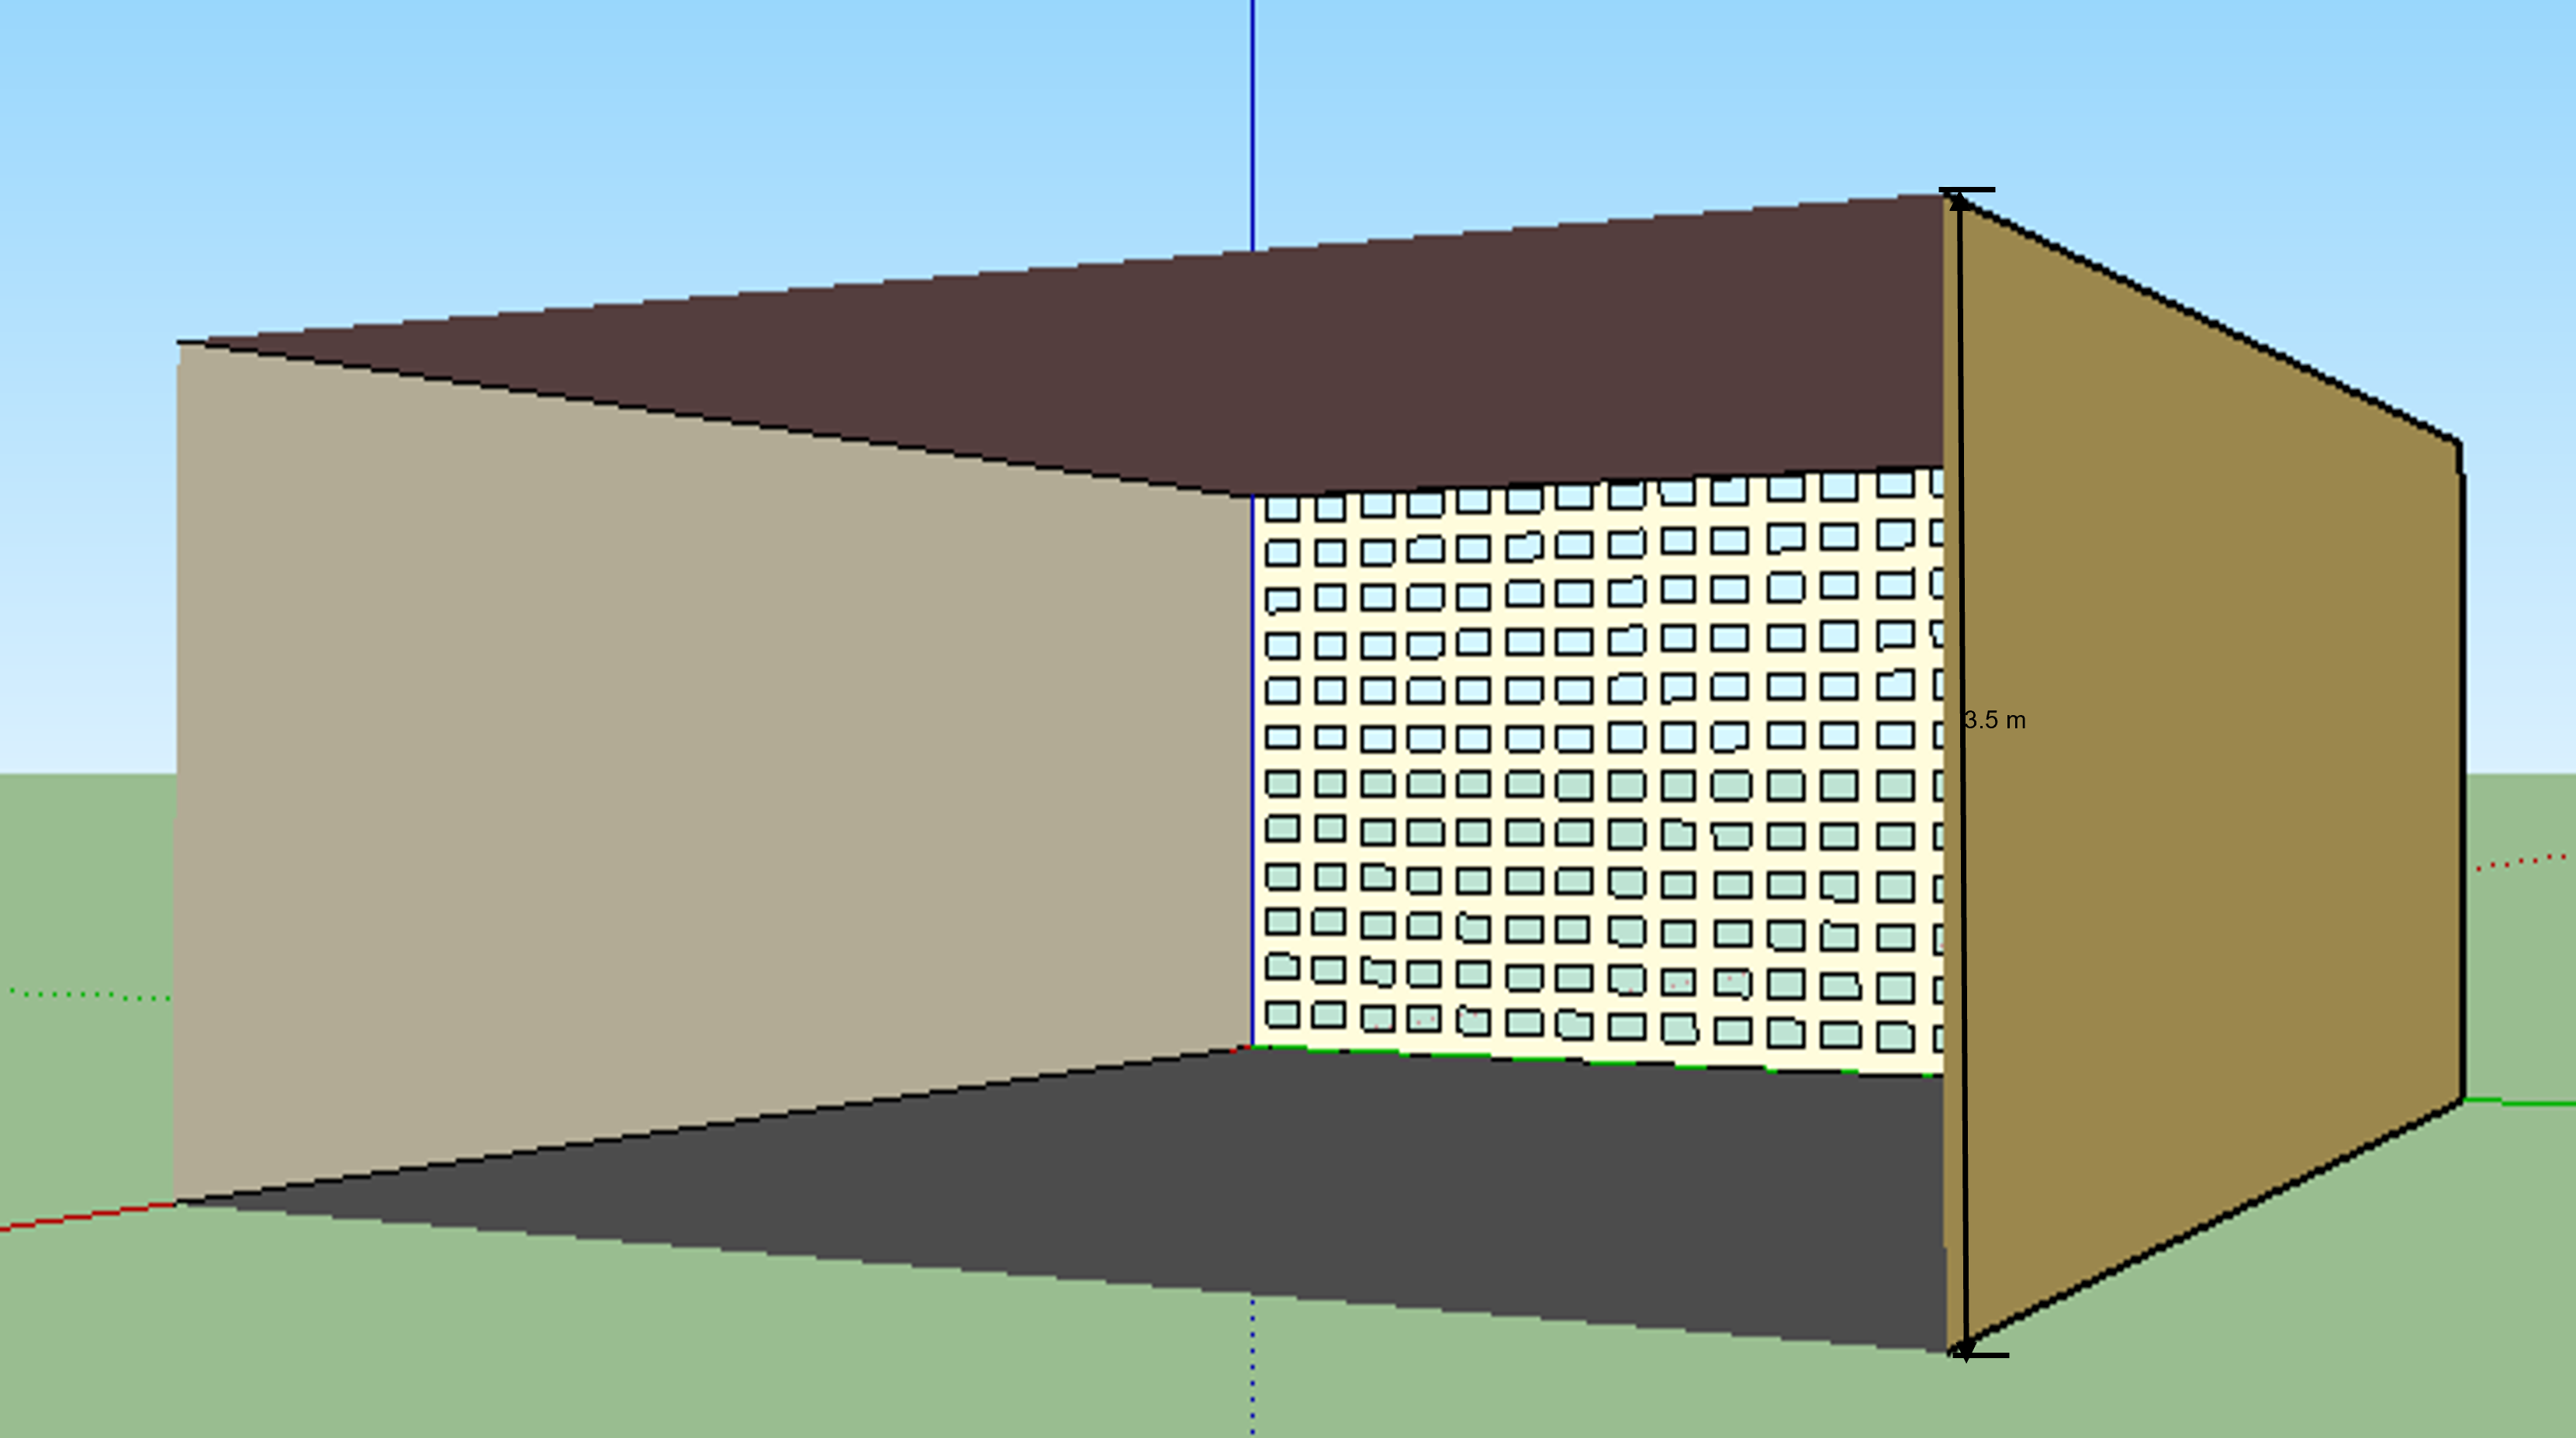
\includegraphics[scale=0.3]{cafeteria_alto_dimesiones.PNG}
\caption{Side view}
\label{fig:Side view}
\end{subfigure}
\caption{Cafeteria dimensions}
\label{fig:Cafeteria dimensions}
\end{figure}


The lattice on the west wall is made up of 264 openings (12x22). The size of each opening is 15x22 cm.

\begin{figure}
 \centering
 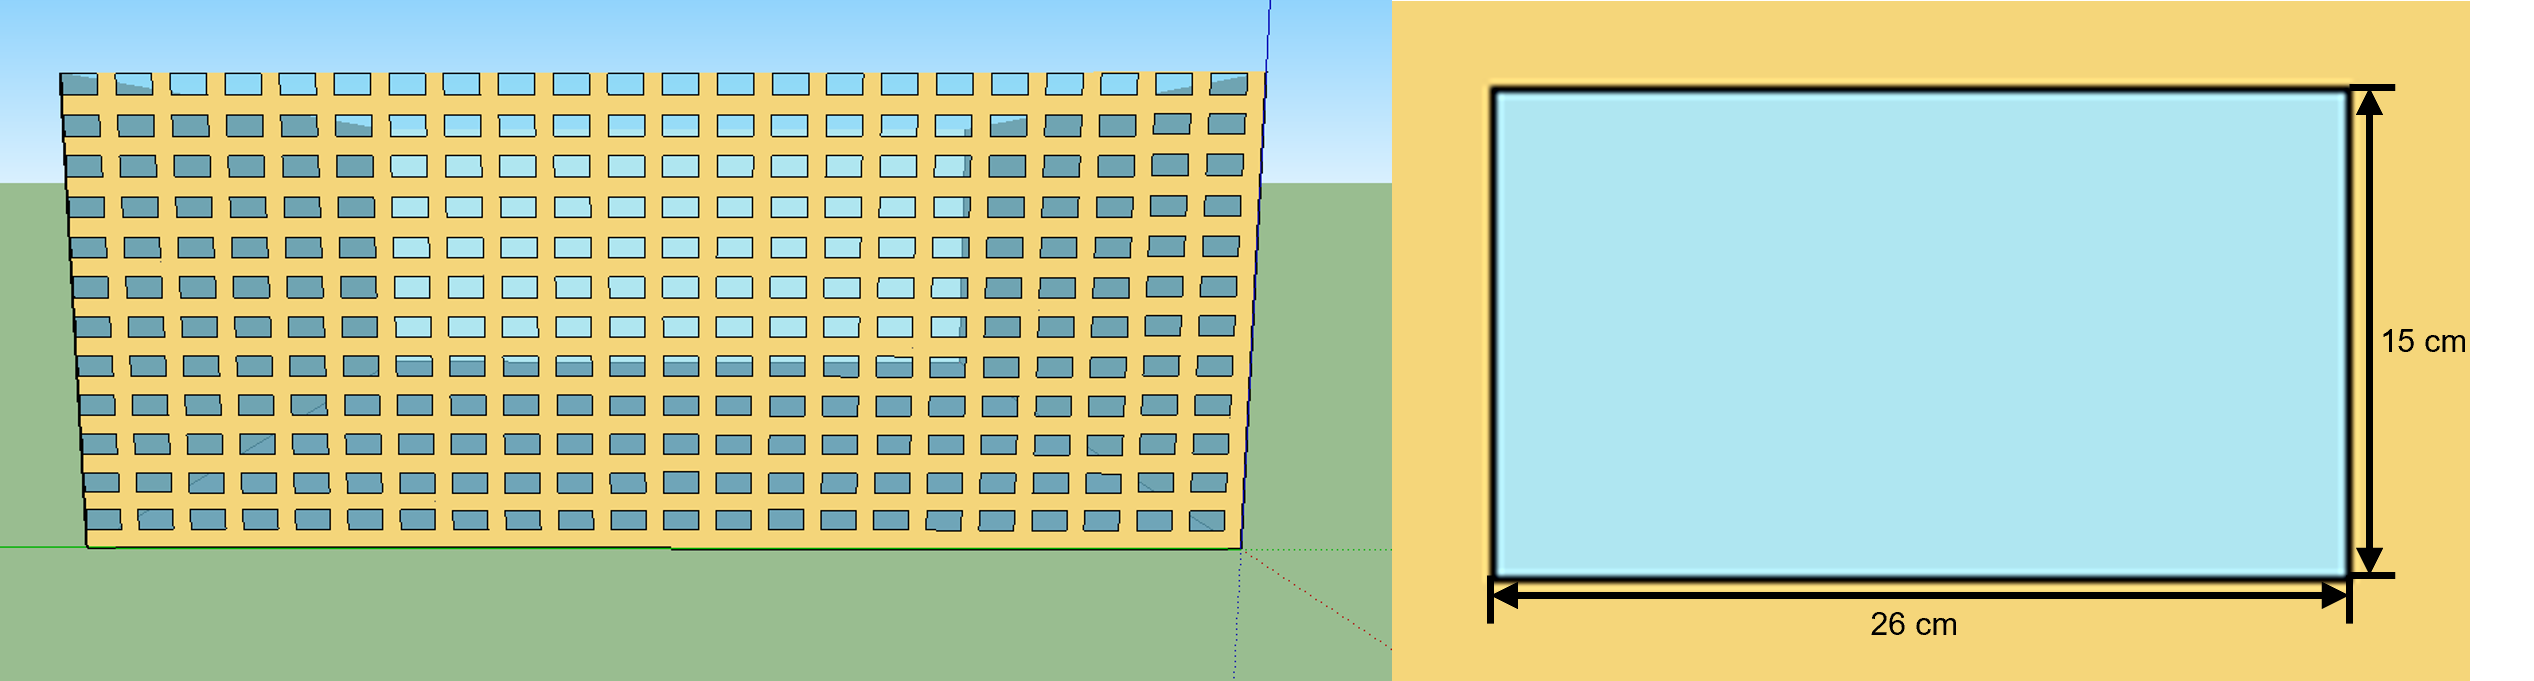
\includegraphics[scale=0.5]{cafeteria_celosia.PNG}
 \caption{West wall
 \label{fig:lattice}
 }
\end{figure}




%Construcción details, materiales, etc

The evaporative cooling in the cafeteria is carried out by an air conditioning system consisting of 30 brass nozzles installed in a nylon pipe circuit. They are installed to the east and west of the cafeteria, at the entrance and next to the lattice. In each part there are 15 nozzles installed at a height of 3.3 m. This system is divided in four subsystems:

\begin{itemize}
\item Filtration system: filters polluting particles from the water and measures water consumption.
\item Nebulization system: it is responsible for the dew drops through a control system that maintains the circulation of water at 6,895 KPa and a flow rate of 1.89 L/min.
\item Thermocouple system: measures the temperature at certain points in the cafeteria
\item Control system: controls the electric valves that allow the circulation of water.
The data acquisition from the sensors is carried out by the thingsboard platform. To carry out the measurements there are three types of sensors: anemometers, thermocouples type T and humidity sensors.
\end{itemize}

\begin{figure}
 \centering
 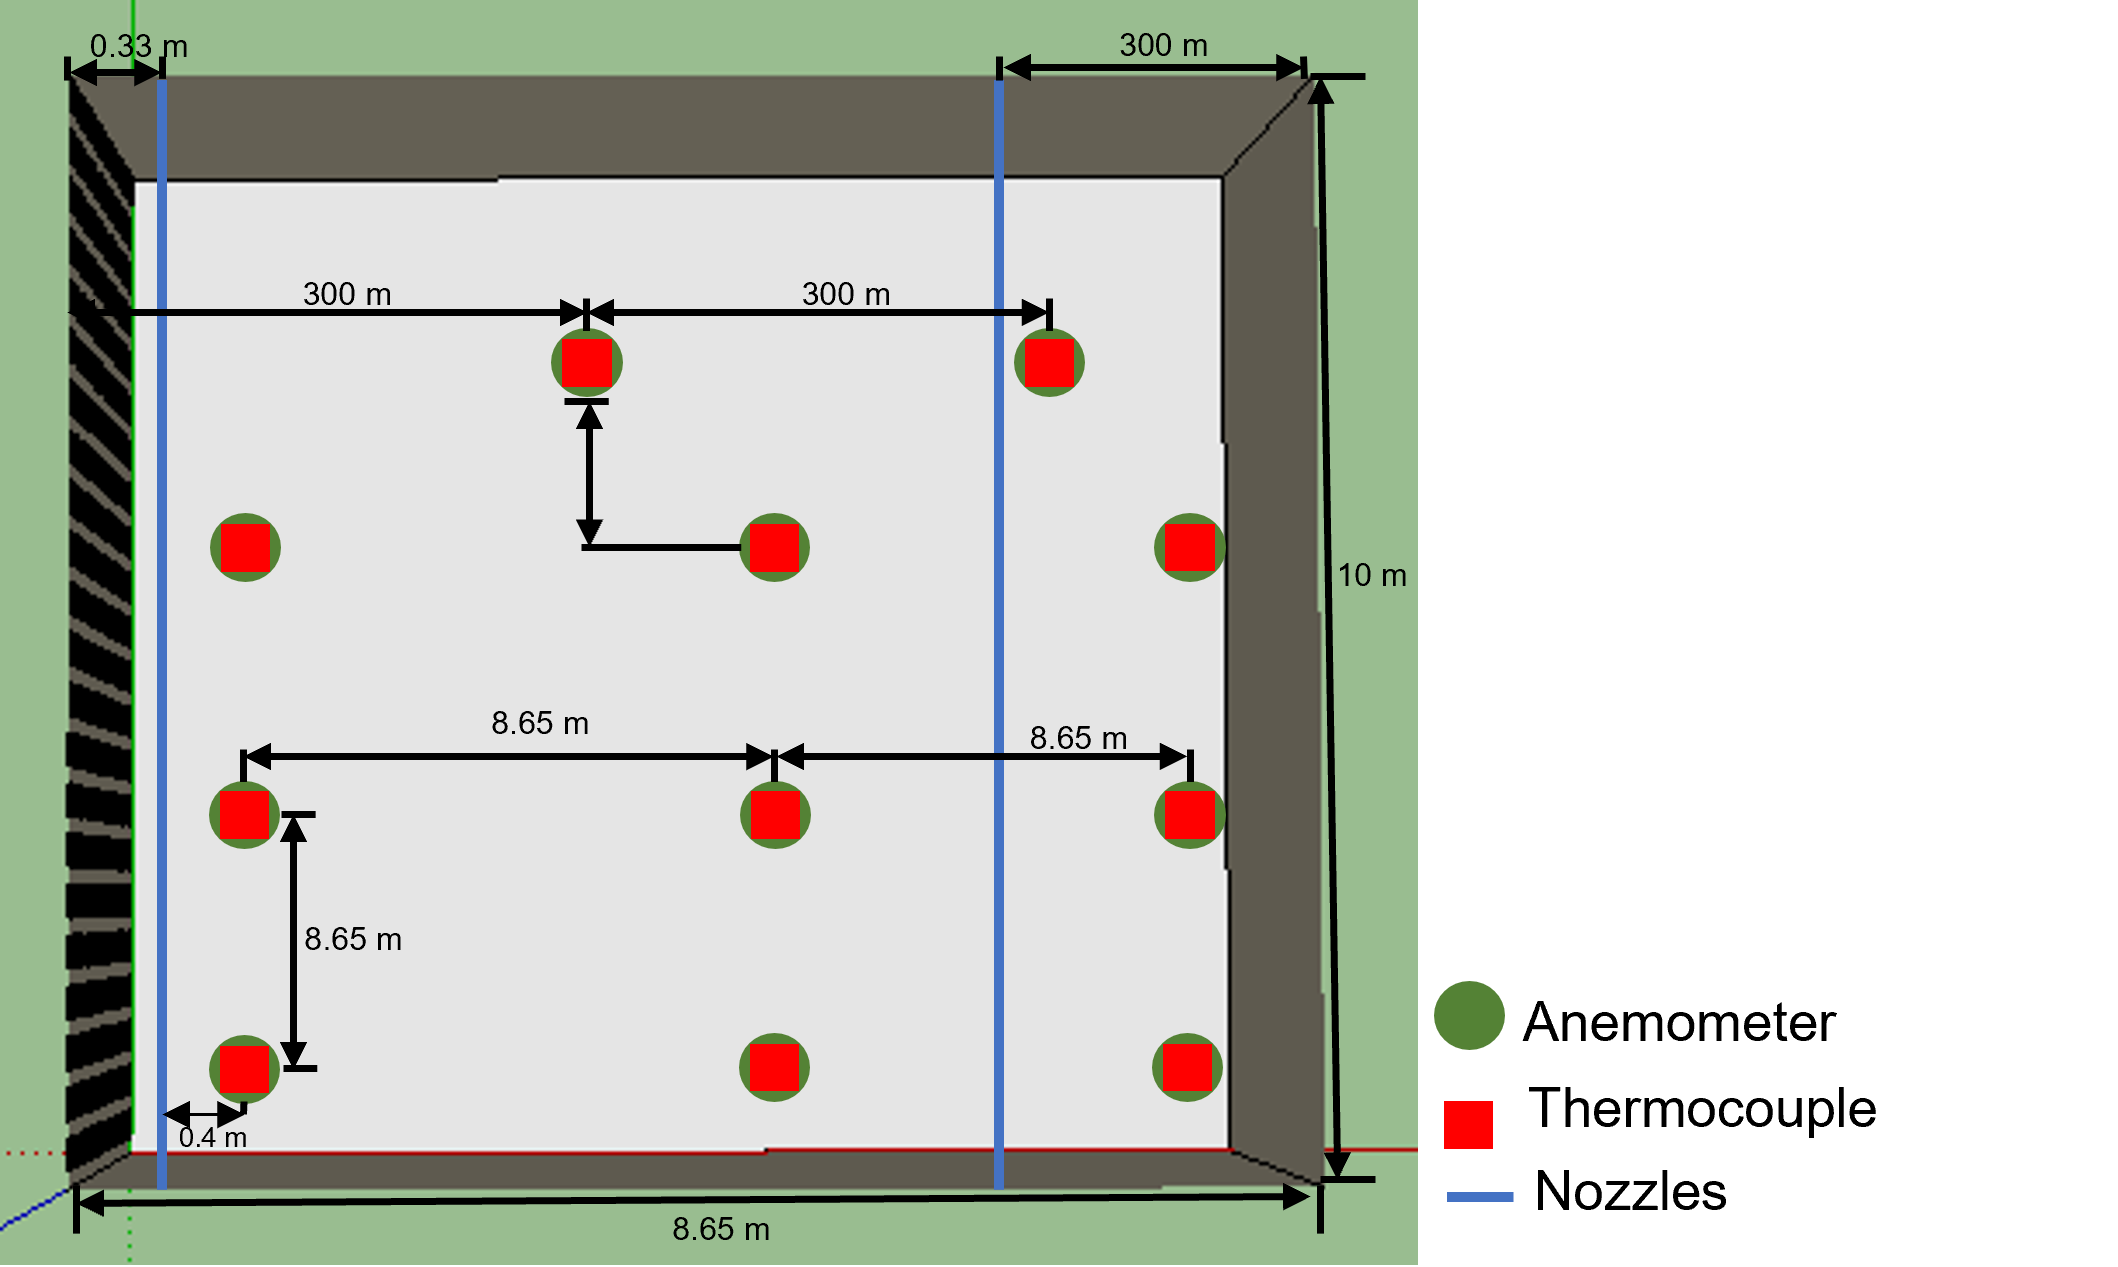
\includegraphics[scale=0.5]{cafeteria_sensores_sketch.PNG}
 \caption{Sensors location
 \label{fig:sensors}
 }
\end{figure}





 
 
 \section{Numerical experiments}
 
 Hay que esperar un poco, pero podría ser numerical simulation and validation… pero ya que tengamos más información lo consideramos.


También hay que considerar si habrá algunos apéndices, reportando tus libretas, me parece interesante documentar tu proceso de aprendizaje.
 
 \section{Validation process}
 
